\chapter{Introduction}

\textbf{\textcolor{red}{THIS THESIS IS CURRENTLY AN UNPUBLISHED DRAFT. IT HAS
NOT BEEN SUBMITTED AND MAY HAVE MISSING CITATIONS AND CONTENT}}

Nuclear structure has been studied since late 19th century, but a complete
understanding of the proton's spin has eluded scientists.  Early models of the
proton structure such as the three valence quark model could accurately predict
the charge and spin of the proton, yet when measured in the late 1980's, was
found to be wrong in an event known as the`proton spin crisis'
(Figure~\ref{fig:spin_crisis_cartoon}).

Although recent papers \cite{Povh2016} have suggested that this `spin crisis'
(Figure~\ref{fig:spin_crisis_cartoon}) is simple due to mis-attribution of
spin, most literature to date has focused on understanding how to model the
proton with parton distribution functions, and the vast scientific consensus is
that the EMC results published detailing the spin crisis in 1988 are valid.

Following the spin crisis, a major challenge in particle physics theory was to
create a framework which could explain both the `valence-quark' behavior of
protons at some scattering energies, as well as predict the break down of that
model and properly account for the proton's spin. Global analyses
~\cite{DeFlorian2009} were undertaken to undertaken to model proton with
probabilistic structure functions, incorporating scale-dependent structure.
These global analyses require experimental data as a constraint for the
structure function parameterization. One method of providing constraints is
through the measurement of particle production asymmetries~\cite{Kang2011}.

Structure functions can be used to calculate parton distribution functions.
Parton distribution functions describe the momentum fraction carried by partons
in the proton. Parton distribution functions may describe either polarized or
unpolarized partons. In global analyses, the parton distribution functions for
quark polarization are estimated, and experimental data constrains these
functions via the calculation of the asymmetry.

\begin{figure}
  \centering
  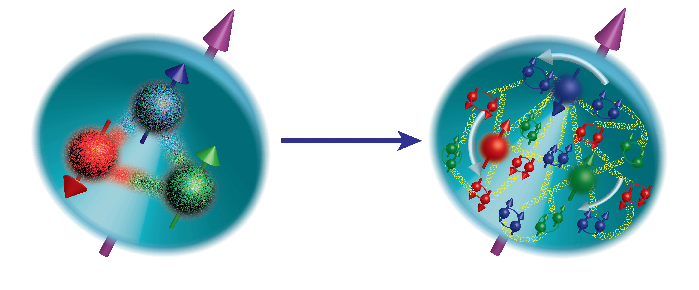
\includegraphics[width=0.8\linewidth]{./figures/figures_introduction_nucleon_picture.png}
  \caption{
    Left: the n{\"a}ive quark model, while predicting the correct spin of the
    proton, does not bear fruit when the quark spin contribution is measured.
    Right: a more realistic cartoon of the proton as a composite of gluons,
    valence quarks and sea-quarks~\cite{Accardi2012}.
  }
  \label{fig:spin_crisis_cartoon}
\end{figure}
 
\section{Scope and Objectives of This Work} 

In the first part of this thesis, I will describe the research I carried out
between May of 2010 through August of 2016.  This analysis comprises the body of
work devoted to calculating $A_L$ for the $W\rightarrow\mu$ decay. The results
of this analysis are used in global fits to constrain the total contribution of
quarks and anti-quarks in the so-called `proton-sea' to the proton's total spin.

In the second portion of this work, I will discuss the `Vernier Analysis', which
is instrumental for every single-cross-section measured with RHIC data.
The thrust of the Vernier Analysis is to determine the beam luminosity at
PHENIX's interaction point. This enables one to normalize the results to the p+p
cross-section. This is done with a series of specialized Vernier-Scans, where
beams are scanned across one-another in order to measure beam geometry. The
luminosity can then be calculated from first principals, and compared to the
estimated machine luminosity published by RHIC's collider-accelerator
department. I produced an entire software framework for handling data cleaning,
analysis, visualization and simulation.
